\section{Энергия магнитного поля системы контуров с током. Коэффициенты само-
и взаимоиндукции. Симметричность матрицы коэффициентов Lik.}

\subsection*{Энергия магнитного поля системы контуров с током}

\textit{Для одного контура:}

Ток I идет по замкнутому контуру.

\begin{gather*}
    \varepsilon=-\frac{1}{c}\frac{d\Phi}{dt}; \qquad \varepsilon_{\text{ист.}}=\frac{1}{c}\frac{d\Phi}{dt} \\
    dW=I\varepsilon_{\text{ист}}dt=I \frac{1}{c}\frac{d\Phi}{dt}=\frac{1}{c}Id\Phi     
\end{gather*}

\textit{Для нескольких контуров:}

\begin{minipage}[c]{0.4\textwidth} % Левая часть: изображение
    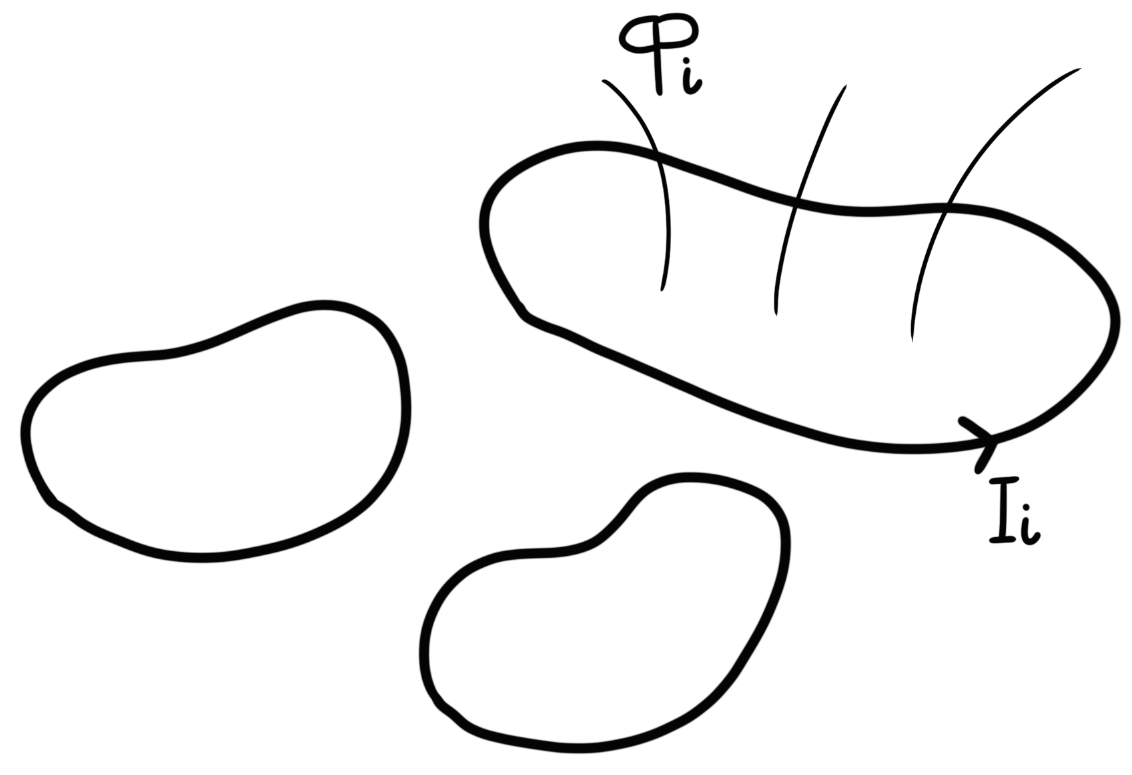
\includegraphics[width=\textwidth]{im/93.png}% Ваше изображение
\end{minipage}%
\hfill
\begin{minipage}[c]{0.6\textwidth} % Правая часть: текст
    \begin{gather*}
        \text{При} I_i=0 \quad W=0 \\
        dW=\frac{1}{c}\sum_{i}I_id\Phi_i 
    \end{gather*}
\end{minipage}

В случае линейной среды:

\[
\tilde{I}_i=\alpha I_i \text{ , где }0\leqslant \alpha\leqslant 1 \Rightarrow \tilde{\Phi}_i=\alpha \Phi_i \text{ и } d\tilde{\Phi}_i=\Phi_i d\alpha
\]

\[
W=\frac{1}{c} \sum_{i}\tilde{I}_id\tilde{\Phi}_i=\frac{1}{c}\sum \int \alpha I_i \Phi_i d\alpha=\sum_{i}\frac{1}{c}\Phi_i I_i \int_{0}^1\alpha d\alpha=\sum \frac{1}{2c}\Phi_i I_i    
\]

В случае линейной среды: \( \boxed{W=\frac{1}{2c}\sum_{i}\Phi_iI_i } \) 

В случае нелинейной среды: \( \boxed{dW=\frac{1}{c}\sum_{i}I_id\Phi_i } \) 

Энергия магнитного поля через: \( \vec{A} and \vec{j} \) 

\[
\text{Поток: } \Phi=\underset{\mathbb{S}}{\iint}\vec{B}d\vec{S}=\underset{\mathbb{S}}{\iint}\mathrm{rot}\vec{A}d\vec{S}=\underset{\delta\mathbb{S}}{\oint}\vec{A}d\vec{l} 
\]

Тогда: \( \frac{1}{2c}\sum_{i}\underset{\mathbb{L}}{\oint}I_i \vec{A}d\vec{l}  \) при переходе к распределенным токам: 

\( Id\vec{l}\rightarrow\vec{j}dV \):

\[
\boxed{W=\frac{1}{2c}\iiint \vec{A}\vec{j}dV }
\]

Аналогично для нелинейной среды: 

\[
\boxed{\delta W=\frac{1}{c}\iiint \vec{j}\delta \vec{A} dV }
\]

\subsection*{Коэффициенты само-
и взаимоиндукции и Симметричность матрицы коэффициентов Lik.}

\[
    \begin{pmatrix}
        \Phi_1 \\
        \Phi_2 \\
        \vdots \\
        \Phi_i \\
        \vdots
        \end{pmatrix}
        =
        \renewcommand{\arraystretch}{1.8} % Увеличивает вертикальные интервалы в матрице
        \setlength{\arraycolsep}{1.2em}   % Увеличивает горизонтальные интервалы между столбцами
        \frac{1}{c} 
        \begin{pmatrix}
           &   &   \\
           & \overset{\wedge}{L} &   \\
           &   &  
        \end{pmatrix}
        \quad
        \renewcommand{\arraystretch}{1.} 
        \setlength{\arraycolsep}{1.2em}   
        \begin{pmatrix}
        I_1 \\
        I_2 \\
        \vdots \\
        I_i \\
        \vdots
        \end{pmatrix}
        \quad
\]

Где \(\overset{\wedge}{L}\) - матрица индуктивных коэффициентов

\[
\Phi_i= \frac{L_{ij}I_i}{c} \quad L_{ij}\text{- коэф. самоиндукции} 
\]

Докажем, что \(  L_{ij}=L_{ji} \):

\begin{gather*}
    \left[ W = \frac{1}{2c}I_i\Phi_i, \; dW = \frac{1}{c}I_i d\Phi_i \right] 
    \Rightarrow \frac{1}{2}d(I_i\Phi_i) = I_i d\Phi_i, \\
    \frac{1}{2}\Phi_i dI_i + \frac{1}{2}I_i d\Phi_i = I_i d\Phi_i 
    \Rightarrow \Phi_i dI_i = I_i d\Phi_i, \\
    \frac{1}{c}L_{ij}I_idI_i=I_iL_{ji}\frac{1}{c}
    \Rightarrow (L_{ij}-L_{ji})I_jdI_i=0 \Rightarrow L_{ij}=L_{ji} \quad \blacksquare 
\end{gather*}

\[
W=\frac{1}{2c^2}L_{ij}I_iI_j 
\]

Для самоиндукции:

\[
W=\frac{1}{2c^2}LI^2 
\]